\documentclass[algorithm,pgfplots]{cuzbeamer}
\usefonttheme{serif}
\setCJKmainfont{Noto Sans CJK SC}
\usepackage[scale=2]{ccicons}

\begin{document}
    \title{Relation Network for Few-shot Learning}
\subtitle{——基于多卡的并行加速}
\date{\today}
\author{刘佳玮,计算机科学与技术学院,20031211496}
\email{https://muyuuuu.github.io}
    \maketitle

    \begin{frame}{大纲}
        \setbeamertemplate{section in toc}[sections numbered]
        \tableofcontents
    \end{frame}

    \section{好的算法与好的设备}

    \begin{frame}{算法时间复杂度}
        \begin{leftbar}
            同一个问题,一个时间复杂度$O(n^2)$与$O(n^3)$的时间对比,代码开放于:
            {\sffamily \url{https://github.com/muyuuuu/Algorithm/tree/master/Insert_sort}}
        \end{leftbar}
        \begin{figure}[h]
            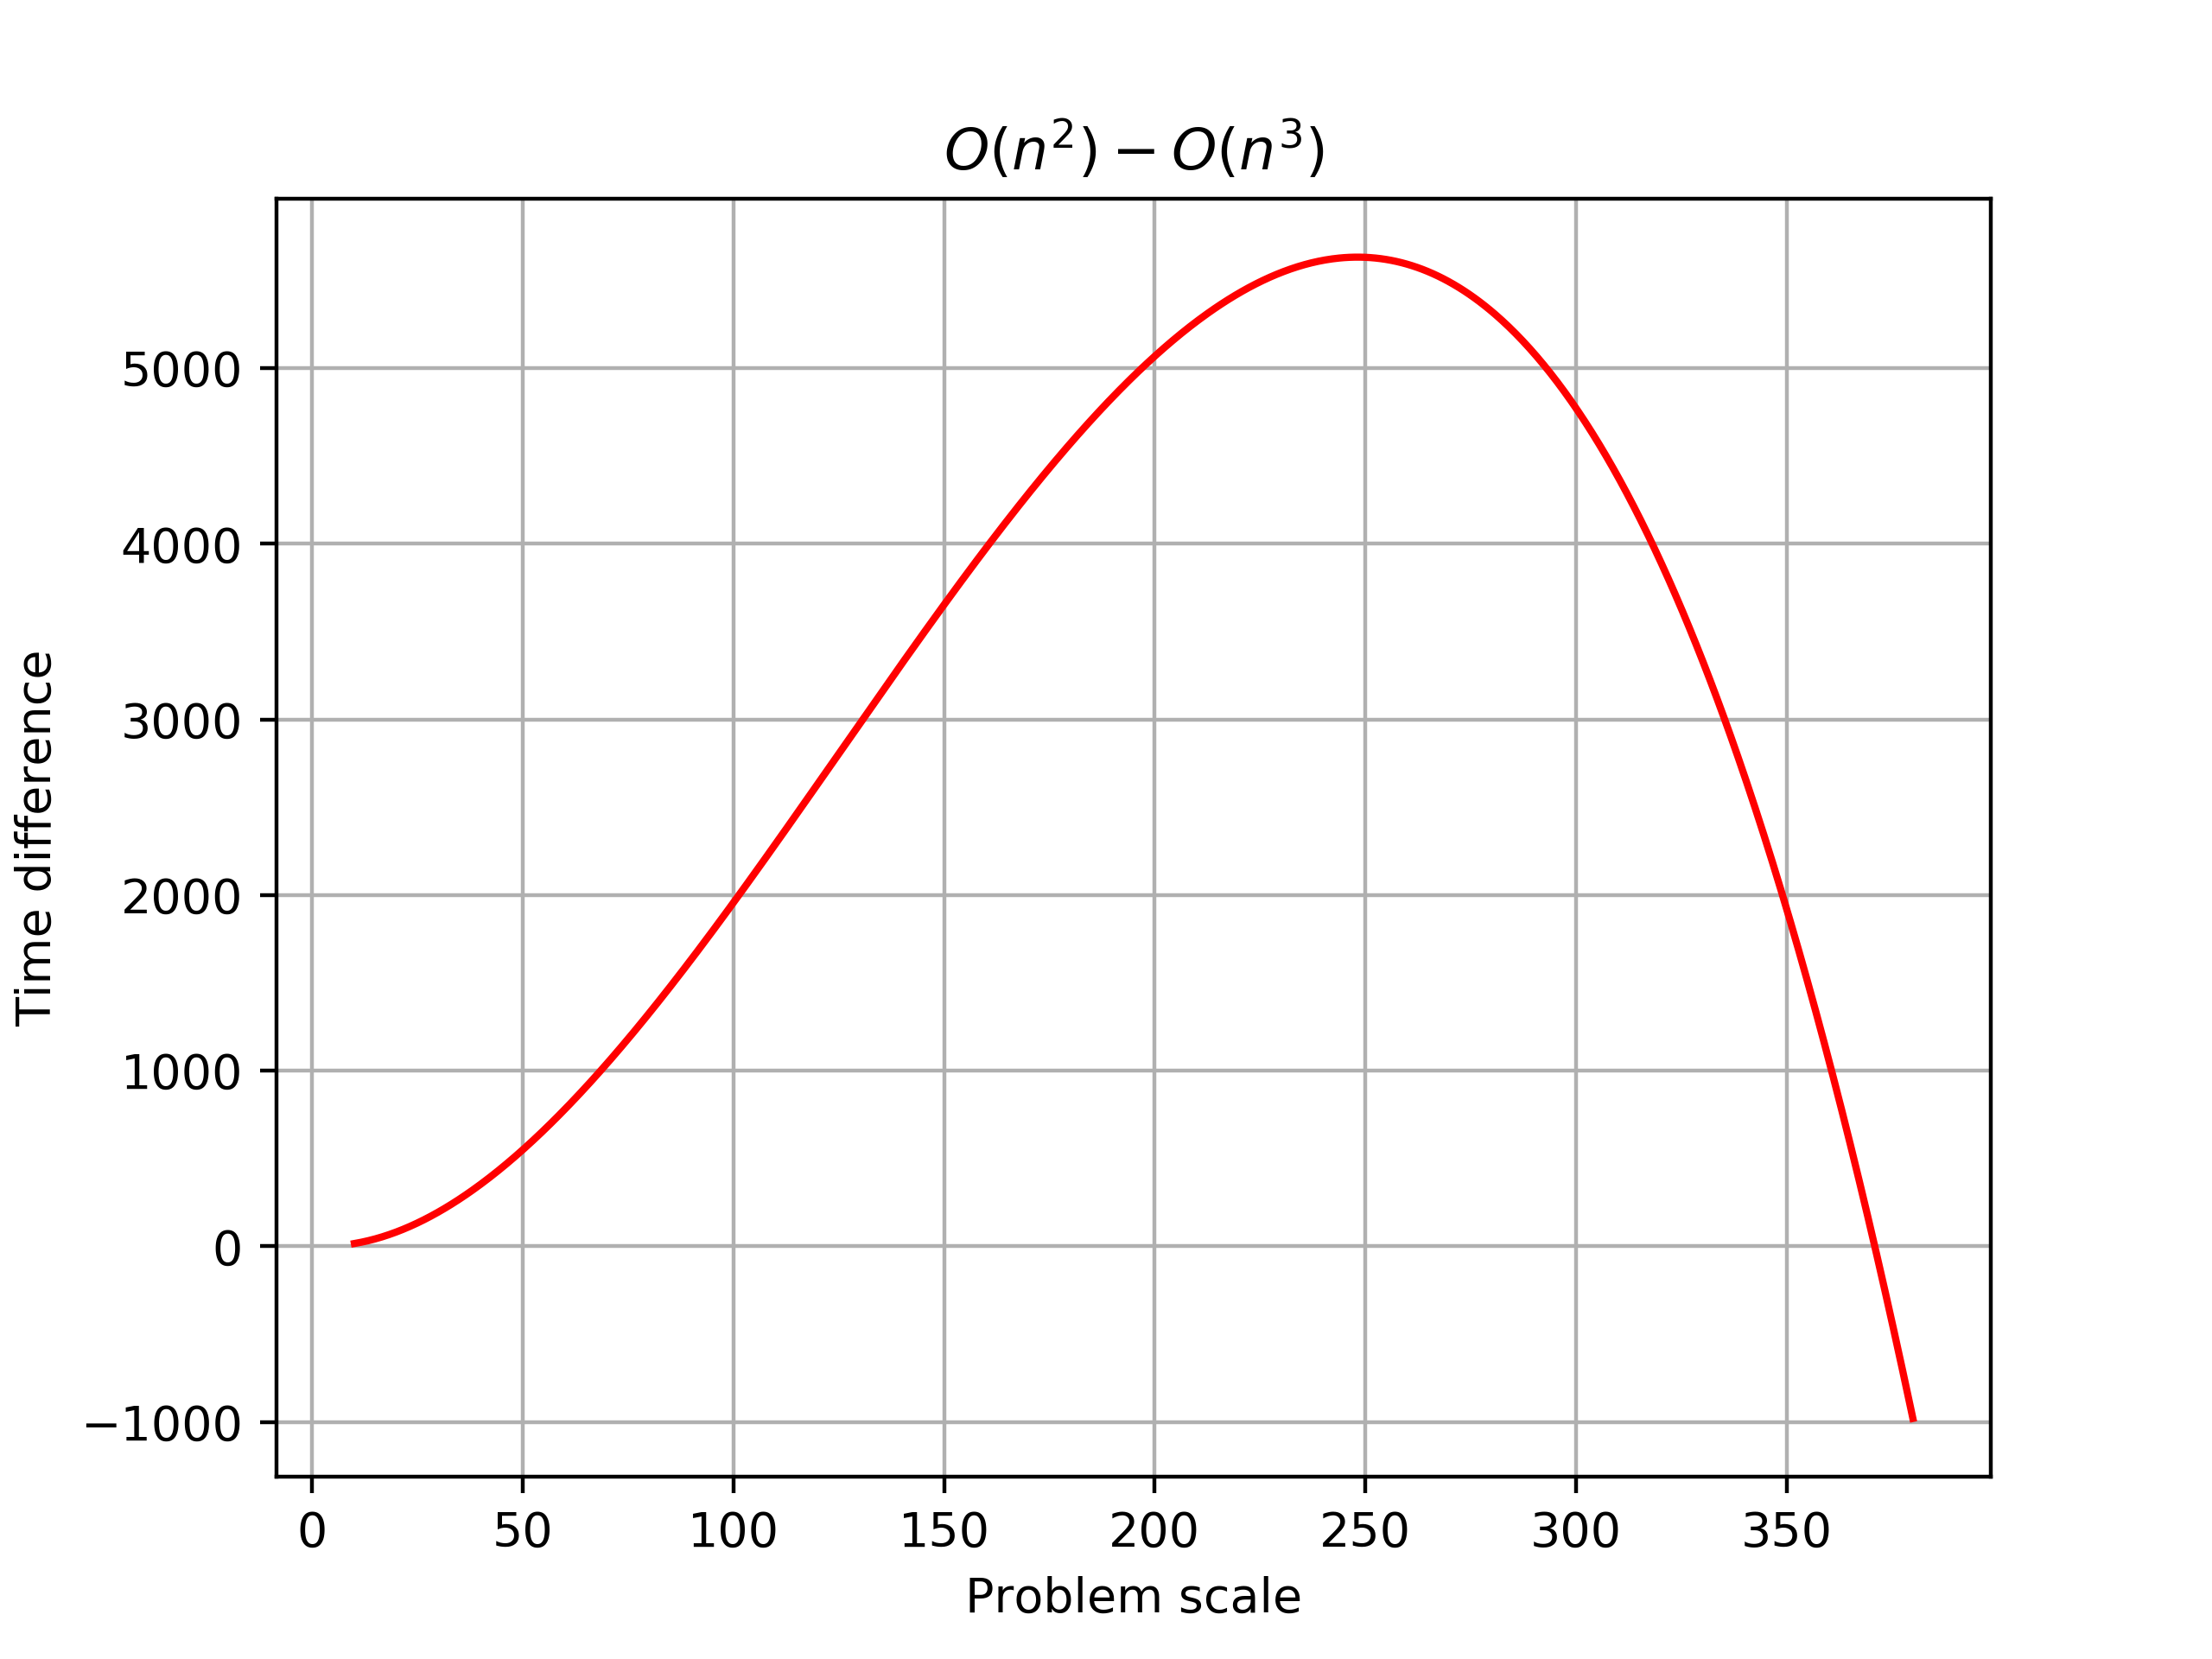
\includegraphics[scale=0.55]{figure/time-complexity.png}
            % \caption{算法时间复杂度的对比}
        \end{figure}
    \end{frame}

    \section{发挥设备优势}

    \begin{frame}{发挥设备优势}
        一个耗时1153秒的单进程任务:
        \begin{figure}[h]
            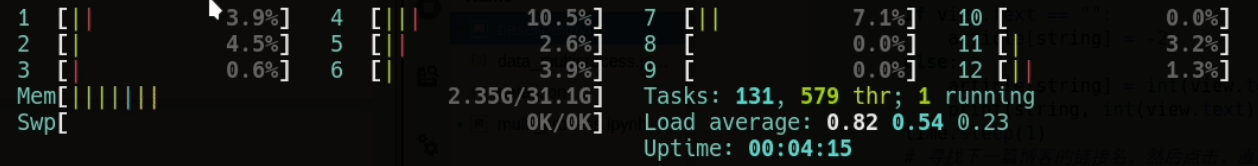
\includegraphics[scale=0.3]{figure/single.png}
            % \caption{单进程执行下的资源利用率}
        \end{figure}
        
        使用多进程改进,相同任务耗时105秒,且多核利用率较为均衡:
        \begin{figure}[h]
            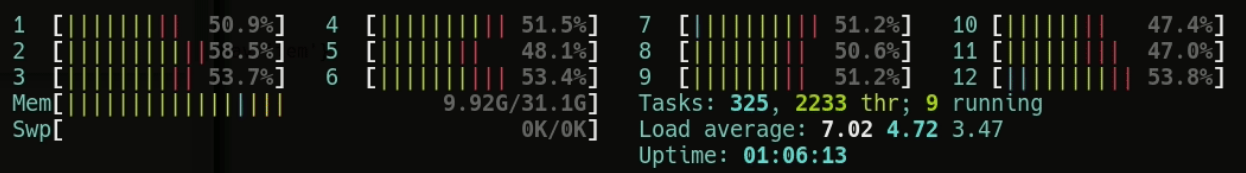
\includegraphics[scale=0.3]{figure/multi.png}
            % \caption{多进程执行下的资源利用率}
        \end{figure}
        
        \begin{leftbar}
        任务必须可以并行化。代码地址:{\sffamily \url{https://muyuuuu.github.io/2020/03/18/multi-process/}}
        \end{leftbar}
        
    \end{frame}

    \section{硬件与软件依赖}

    \begin{frame}{硬件与软件}
        \metroset{block=fill}
        \begin{exampleblock}{硬件部分}
            \begin{description}
                \item[{\ttfamily CPU}] 2个Intel(R) Xeon(R) Gold 5115 CPU \@ 2.40GHz,10核心20线程
                \item[{\ttfamily GPU}] 4路Tesla P40,每路显存容量22GB
                \item[内存] 128GB
                \item[外存] 520TB可用,已用15TB
            \end{description}
        \end{exampleblock}
        \metroset{block=fill}
        \begin{exampleblock}{软件部分}
            \begin{description}
                \item[系统] CentOS Linux release 7.3.1611 (执行), Arch 5.9.6(开发)
                \item[{\ttfamily python}] 3.8.2,开发语言
                \item[{\ttfamily pytorch}] 1.6.0,模型实现,借助其提供的API实现并行
                \item[{\ttfamily ssh}] OpenSSH\_8.3p1, OpenSSL 1.1.1h:实现远程登录
                \item[{\ttfamily scp}] 文件传输
            \end{description}
        \end{exampleblock}
    \end{frame}

    \begin{frame}{常用命令}
        \begin{alertblock}{命令行内执行}
            \begin{enumerate}
                \item {\ttfamily mv, cd, ls, cp, cat} 等文件操作
                \item {\ttfamily nohup python train.py > log} 挂起运行与重定向输出
                \item {\ttfamily ps -f|grep python} 查看挂起程序是否执行
            \end{enumerate}
        \end{alertblock}
    \end{frame}

    \section{模型}

    \begin{frame}{模型结构}
        \begin{leftbar}            
            实现的模型为Relation Network\footnote{\sffamily{\url{https://ieeexplore.ieee.org/abstract/document/8778601}}}。
            数据集为miniImageNet\footnote{\sffamily{\url{https://drive.google.com/file/d/0B3Irx3uQNoBMQ1FlNXJsZUdYWEE/view}}}。
        \end{leftbar}
        \begin{figure}[h]
            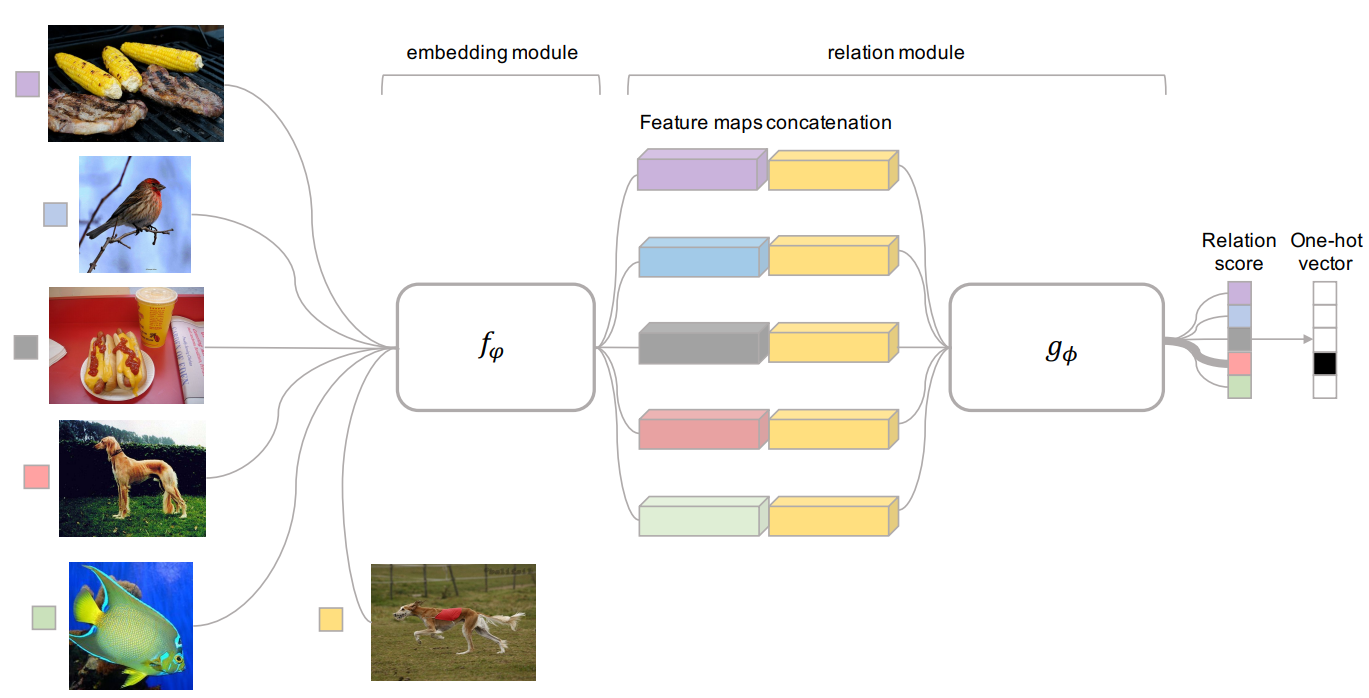
\includegraphics[scale=0.24]{figure/compare.png}
            % \caption{Relation Network结构图}
            % \label{fig:compare}
        \end{figure}
    \end{frame}

    \begin{fragile}[最终模型结构]
        \begin{leftbar}
            共计 11,285,569 个参数,约75MB左右的参数。
        \end{leftbar}
        \bicolumns[0.0]{
        }{
            \begin{block}{13组特征提取模块,7组连接处理模块}
                \begin{minted}{python}
                (conv1): Conv2d(64, 64, kernel_size=(1, 1), stride=(1, 1), bias=False)
                (bn1): BatchNorm2d(64, eps=1e-05, momentum=0.1, affine=True)
                (conv2): Conv2d(64, 64, kernel_size=(3, 3), stride=(1, 1), padding=(1, 1), bias=False)
                (bn2): BatchNorm2d(64, eps=1e-05, momentum=0.1, affine=True)
                (conv3): Conv2d(64, 256, kernel_size=(1, 1), stride=(1, 1), bias=False)
                (bn3): BatchNorm2d(256, eps=1e-05, momentum=0.1, affine=True)
                (relu): ReLU(inplace=True)
                (0): Conv2d(64, 256, kernel_size=(1, 1), stride=(1, 1), bias=False)
                (1): BatchNorm2d(256, eps=1e-05, momentum=0.1, affine=True)
                \end{minted}
            \end{block}
            \begin{block}{1组计算相关性模块}
                \begin{minted}{python}
                (0): Linear(in_features=256, out_features=64, bias=True)
                (1): BatchNorm1d(64, eps=1e-05, momentum=0.1, affine=True)
                (2): ReLU(inplace=True)
                (3): Linear(in_features=64, out_features=1, bias=True)
                (4): Sigmoid()
                \end{minted}
            \end{block}
        }
    \end{fragile}

    \section{并行实现}

    \begin{frame}{多角度并行}
        \begin{leftbar}
            保持实验参数一致。
        \end{leftbar}
        \metroset{block=fill}
        \begin{block}{并行加载数据}
            \begin{enumerate}
                \item {\ttfamily DataLoader},{\ttfamily num\_workers}指定加载数据进程的
                数量。
                \item {\ttfamily .cuda()} 在指定设备上设置和运行CUDA操作,使其支持CUDA张量类型;
                之后便可以使用GPU完成计算。
            \end{enumerate}
        \end{block}

        \metroset{block=fill}
        \begin{block}{并行训练模型}
            \begin{enumerate}
                \item 单机单卡
                \item 单机多卡
                \item 多机多卡
            \end{enumerate}
        \end{block}
    \end{frame}

    \begin{frame}{并行实现}
        \begin{leftbar}
            模型过大,因此不进行CPU实验和GPU单卡实验,只对比单机多卡或多机多卡下不同并行方式的加速比。
        \end{leftbar}
        \metroset{block=fill}
        \begin{block}{ }
            \begin{itemize}
                \item {\ttfamily DataParallel\footnote{\ttfamily https://pytorch.org/docs/stable/generated/torch.nn.DataParallel.html}}
                ,给定模型,将输入划分给不同的设备。
                前向计算阶段,每个设备复制一份模型,读取自己的输入并执行;反向传播阶段,每个设备的loss汇总到原始模型(指定设备的模型),计算梯度并重新分配下去。
                \item {\ttfamily DistributedDataParallel\footnote{\ttfamily https://pytorch.org/tutorials/intermediate/ddp\_tutorial.html}},
                DDP 使用集群通信来同步梯度和缓冲区的数据。DDP 对模型中每一个可求导的参数申请一个钩子,
                当对应的参数在反向传播中计算梯度时,钩子会触发信号,DDP发射信号后来同步不同的进程间的数据\footnote{\ttfamily \url{https://pytorch.org/tutorials/intermediate/dist_tuto.html}},阻塞等待所有参数更新完毕。
            \end{itemize}
        \end{block}
    \end{frame}

    \begin{fragile}[DataParallel与DistributedDataParallel对比]
        \begin{columns}[T,onlytextwidth]
            \column{0.4\textwidth}
            \metroset{block=fill}
            \begin{block}{DistributedDataParallel}
                \begin{itemize}
                    \item 多进程实现
                    \item 支持多机
                    \item 支持模型并行,将模型拆分,并放到多个机器
                    \item 通信方式:{\ttfamily Allreduce} 
                \end{itemize}
            \end{block}
            \column{0.4\textwidth}
            \metroset{block=fill}
            \begin{block}{DataParallel}
                \begin{itemize}
                    \item 单进程多线程实现,由于GIL锁的存在,效率低下
                    \item 只能用于单机
                    \item 通信方式:scattering inputs and gathering outputs.
                \end{itemize}
            \end{block}
        \end{columns}
    \end{fragile}

    \begin{fragile}[并行部分伪代码]
        \begin{columns}[T,onlytextwidth]
            \column{0.9\textwidth}
            \begin{block}{设备检测,即如何监测多卡}
                \begin{minted}{python}
                    if device_ids is None:
                        device_ids = _get_all_device_indices()

                    if output_device is None:
                        output_device = device_ids[0]
                \end{minted}
            \end{block}
            \begin{block}{DataParallel}
                \begin{minted}{python}
                    net = DataParallel(Compare(n_way, k_shot)).cuda()
                \end{minted}
            \end{block}
            \begin{block}{DistributedDataParallel}
                \begin{minted}{python}
                    1. initialize the process group
                    2. net = DDP(Compare(n_way, k_shot).to(rank), device_ids=[rank])
                    3. destroy_process_group
                \end{minted}
            \end{block}
        \end{columns}
    \end{fragile}

    \section{实验结果}
    
    \begin{frame}{DataParallel 单机多卡}
        \begin{leftbar}
            {\ttfamily nvidia-smi}查看显卡利用率:
        \end{leftbar}
        \begin{figure}
            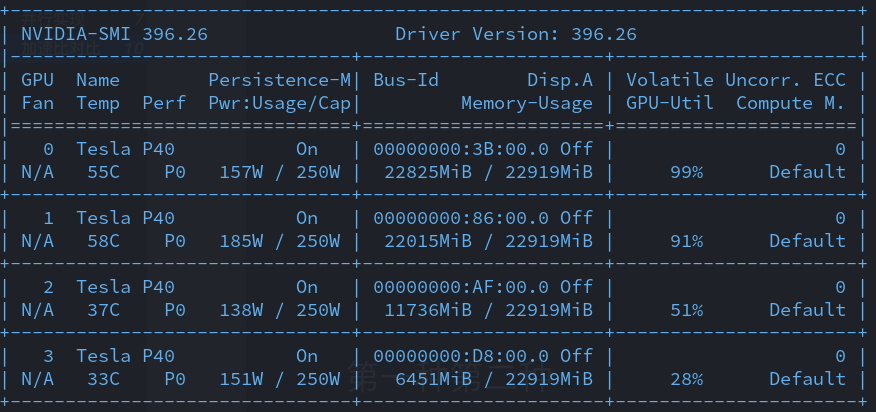
\includegraphics[scale=0.4]{figure/01gpu-use.png}
        \end{figure}
        程序执行时间:$T_1=137172$秒,约2286分钟,约1.59天。
    \end{frame}

    \begin{frame}{DistributedDataParallel 单机多卡}
        \begin{leftbar}
            {\ttfamily nvidia-smi}查看显卡利用率:
        \end{leftbar}
        \begin{figure}
            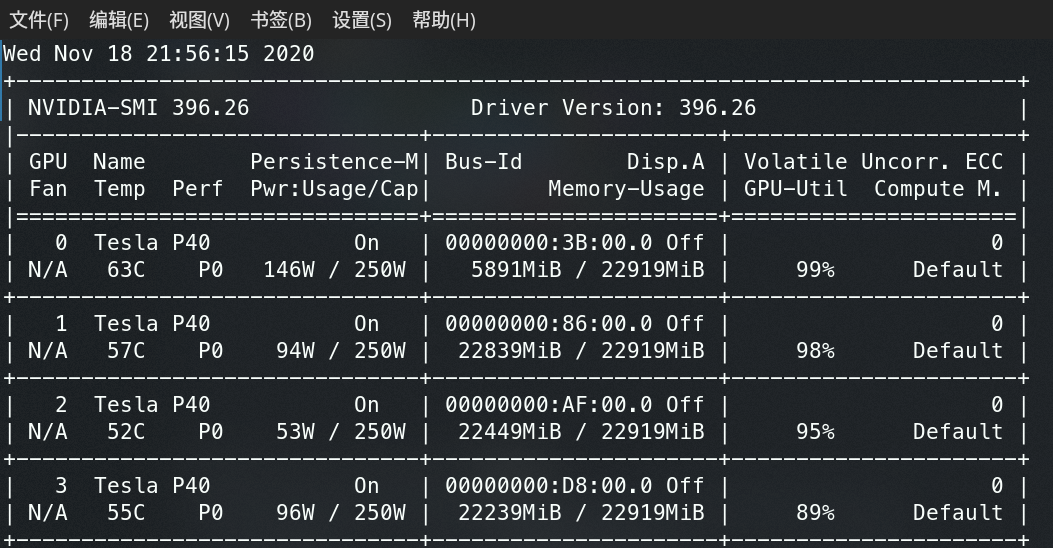
\includegraphics[scale=0.45]{figure/ddp.png}
        \end{figure}
        程序执行时间:$T_2=89856$秒,约1498分钟,约1.03天。
    \end{frame}

    \begin{frame}{DistributedDataParallel 单机多卡}
        \begin{leftbar}
            加速比:$\frac{T_1}{T_2}=1.53$
        \end{leftbar}
        \begin{leftbar}
            准确率对比:Dataparallel:0.566, DDP:0.582。
        \end{leftbar}
        \begin{leftbar}
            代码开放于:{\ttfamily \url{https://github.com/muyuuuu/Algorithm/tree/master/meta-learning/Metric-based/Relation-Netowrk}}
        \end{leftbar}
    \end{frame}


    % \begin{frame}
    %     \begin{columns}[T,onlytextwidth]
    %         \column{0.33\textwidth}
    %         \begin{block}{普通标题}
    %             \begin{itemize}
    %                 \item 普通内容
    %                 \item 普通内容
    %                 \item 普通内容
    %             \end{itemize}
    %         \end{block}
            % \metroset{block=fill}
            % \begin{block}{普通标题}
            %     \begin{itemize}
            %         \item 普通内容
            %         \item 普通内容
            %         \item 普通内容
            %     \end{itemize}
            % \end{block}
    %         \column{0.33\textwidth}
    %         \begin{alertblock}{警告标题}
    %             \begin{enumerate}
    %                 \item 警告内容
    %                 \item 警告内容
    %                 \item 警告内容
    %             \end{enumerate}
    %         \end{alertblock}
    %         \metroset{block=fill}
    %         \begin{alertblock}{警告标题}
    %             \begin{enumerate}
    %                 \item 警告内容
    %                 \item 警告内容
    %                 \item 警告内容
    %             \end{enumerate}
    %         \end{alertblock}
    %         \column{0.33\textwidth}
    %         \begin{exampleblock}{例子标题}
    %             \begin{description}
    %                 \item[描述定义] 描述内容
    %                 \item[描述定义] 描述内容
    %                 \item[描述定义] 描述内容
    %             \end{description}
    %         \end{exampleblock}
    %         \metroset{block=fill}
    %         \begin{exampleblock}{例子标题}
    %             \begin{description}
    %                 \item[描述定义] 描述内容
    %                 \item[描述定义] 描述内容
    %                 \item[描述定义] 描述内容
    %             \end{description}
    %         \end{exampleblock}
    %     \end{columns}
    % \end{frame}

    % \begin{fragile}
    %     \bicolumns{
    %         \begin{block}{图片}
    %             \begin{center}
    %                 % \includegraphics[width=0.65\textwidth]{cuzlogo}\\
    %                 % \includegraphics[width=0.65\textwidth]{cuzlogo-dark}\\
    %                 % \includegraphics[width=0.65\textwidth]{cuzlogo-light}\\
    %                 % \includegraphics[width=0.65\textwidth]{cuzlogo-brown}\\
    %             \end{center}
    %         \end{block}
    %     }{
    %     \begin{block}{表格}
    %         \begin{table}\small
    %             \begin{tabular}{llr}
    %                 \toprule
    %                 \multicolumn{2}{c}{项目} & \multirow{2}{*}{价格 (\$)} \\
    %                 \cmidrule(r){1-2}
    %                 动物                    & 描述 &  \\
    %                 \midrule
    %                 \multirow{2}{*}{蚋蚊}   & 每克 & 13.65 \\
    %                                         & 每只 & 0.01 \\
    %                 角马                    & 标本 & 92.50 \\
    %                 鸸鹋                    & 标本 & 33.33 \\
    %                 犰狳                    & 冷冻 & 8.99 \\
    %                 \bottomrule
    %             \end{tabular}
    %         \end{table}
    %     \end{block}
    %     }
    % \end{fragile}

    % \begin{fragile}[]
    %     \bicolumns[0.382]{
    %     }{
    %         \begin{block}{代码}
    %             \begin{minted}{c++}
    %                 // 西加加
    %                 #include <iostream>

    %                 auto main(int argc, char const **argv) {
    %                     std::cout << "Test" << std::endl;
    %                     return 0;
    %                 }
    %             \end{minted}
    %             \begin{minted}{java}
    %                 // 爪哇
    %                 public class Test {
    %                     public static void main(String[] args) {
    %                         System.out.println("Test");
    %                     }
    %                 }
    %             \end{minted}
    %             \begin{minted}{python}
    %     if device_ids is None:
    %         device_ids = _get_all_device_indices()

    %     if output_device is None:
    %         output_device = device_ids[0]
    %             \end{minted}
    %         \end{block}
    %     }
    % \end{fragile}

    % \begin{fragile}[]
    %     \bicolumns[0.382]{
    %     }{
    %         \begin{block}{算法}
    %             \begin{algorithmx}[alg:euclid]{Euclid算法}
    %                 \Procedure{Euclid}{$a,b$}\Comment{$a$与$b$的最大公约数}
    %                 \State $r\gets a\bmod b$
    %                 \While{$r\neq 0$}\Comment{若$r$为0则可跳出循环返回答案}
    %                 \State $a\gets b$
    %                 \State $b\gets r$
    %                 \State $r\gets a\bmod b$
    %                 \EndWhile\label{euclidendwhile}
    %                 \State \textbf{return} $b$\Comment{最大公约数为$b$}
    %                 \EndProcedure
    %             \end{algorithmx}
    %         \end{block}
    %     }
    % \end{fragile}

    \begin{standout}[]
        感谢聆听!
    \end{standout}

\end{document} 